\documentclass[11pt]{article}
\usepackage{acl-hlt2011}
\usepackage{times}
\usepackage{latexsym}
\usepackage{amsmath}
\usepackage{amsfonts}
\usepackage{multirow}
\usepackage{url}
\usepackage{graphicx}
\usepackage[labelfont=bf]{caption}
\usepackage{verbatim}
\usepackage{algorithm}
\usepackage{algorithmicx}
\usepackage{algpseudocode}
\usepackage{etoolbox}
\usepackage{CJK}

\DeclareMathOperator*{\argmax}{arg\,max}
\setlength\titlebox{4cm}    % Expanding the titlebox

\title{	Native Language Attribution in a Transcribed Speech Corpus}
\author{Bradley Beth \hspace{1em} Nathan Clement\\ 
The University of Texas at Austin \\
{\tt \{bbeth,nclement\}@cs.utexas.edu}\\May 1, 2012}


\begin{document}
\maketitle{}
\begin{abstract}
%% BB
In this paper, we apply statistical machine learning techniques for native language identification (NLI) to a novel dataset---a transcribed speech corpus. Our approach leverages previous work on NLI with text corpora, adjusting for features common to spontaneous speech.  Finally, we evaluate our methodology through 13-way multiclass categorization using support vector machines.
\end{abstract}
\section{Introduction}
% BB
% Motivate and abstractly describe the problem you are addressing and how you are addressing it. What is the problem? Why is it important? What is your basic approach? A short discussion of how it fits into related work in the area is also desirable. Summarize the basic results and conclusions that you will present. 
Authorship attribution is a common application of Natural Language Processing (NLP) and Machine Learning (ML) techniques. As a subfield of text categorization, typical approaches involve the discovery and markup of measurable features within a text (such as stylometry, orthography, and statistical distributions of character, word, or phrasal occurrences) and the application of a statistical classifier over the resulting feature vectors. 

The general problem of authorship attribution has a long history. Mosteller and Wallace \shortcite{Mosteller_Wallace_1964} applied statistical inference to twelve of \emph{The Federalist Papers} in order to resolve disputed authorship claims among historians. Foster \shortcite{Foster2000} applies similar techniques to a variety of authorship disputes, including the authentication of various works of Shakespeare as well as identifying the Unabomber as Ted Kaczynski through textual analysis.

Recent work explores the extension of specific authorship attribution to generalized classification of authors among mutually exclusive categories. Researchers have successfully applied ML to broadly group texts by authors' gender \cite{10.1109/CSAC.2002.1176299}, personality \cite{Nowson2007}, and nationality \cite{Argamon_Levitan_2004}.

Work on Native Language Identification (NLI) is particularly relevant as a potential tool for intelligence gathering and threat identification. Speech processing research has targeted NLI on the basis of acoustic variation for years \cite{Kat_Fung_Bay_Kong_1999,Ahmed_Tan_2011}, but the application of grammatical analysis of text for NLI is relatively recent.  The seminal work using this approach \cite{Koppel2005a} and follow-up studies \cite{Tsur2007,Brooke2012} achieve significant results in classifying L1s (up to 93.8\% accuracy using the \emph{International Corpus of Learner English (ICLE)} \cite{ICLEv2}). This is not entirely surprising; language education researchers have long known that the influence of L1s on future language acquisition leads to residual artifacts that inhibit fluency \cite{Mohan_Lo_1985,Yamashita_Jiang_2010}.

However, Brooke and Hirst \shortcite{Brooke2012} suggest that the results achieved using \emph{ICLE} are biased by the structure of the corpus---particularly its strict topicalization. They demonstrate that a classifier trained on \emph{ICLE} does poorly when validated on \emph{Lang-8} \shortcite{lang-8}, a less formal collection of English as a Foreign Language (ELF) text, and that even the feature set utilized in training \emph{ICLE} does not translate as well to \emph{Lang-8} when cross-validated as a single corpus (an accuracy of 25\% \emph{vs.} 93.8\%).

We propose utilizing a similar methodology to the original approach taken by Koppel, et. al. \shortcite{Koppel2005a}, but applied to a noisy corpus of transcribed \emph{speech}, rather than written text. We are able to achieve an accuracy surpassing that of Brooke and Hirst over the \emph{Lang-8} text corpus (30.8\% \emph{vs.} 25\%).
\section{Problem Definition and Algorithm}

\subsection{Task Definition}
% BB
% Precisely define the problem you are addressing (i.e. formally specify the inputs and outputs). Elaborate on why this is an interesting and important problem. 
Although application of ML to NLI on both speech and text corpora has been studied, to our knowledge, no research exists on the intersection of the two---namely, application of grammatical and lexical analysis to extemporaneous speech. Our work addresses this vacuity through applying techniques developed for text corpora on the \emph{transcriptions} of a speech corpus: the 1 million word Vienna-Oxford International Corpus of English \cite{VOICE}. 

VOICE represents 50 different L1 language backgrounds spread over 1,250 different speakers. Each of the files in the corpus contains L2 English speech. Transcriptions of speech events in the corpus are XML-formatted to document organizational information (e.g., speaker characteristics, including L1) as well as linguistic metadata (e.g., markup of onomatopoeia and word fragments). This allows capture of ``para-linguistic'' phenomena (e.g., pauses and disfluencies, such as the discourse particle `uh') as features as well as semantically relevant words. 

The novelty of this dataset is compounded by its use of conventionalized spelling \cite{VOICEConv}. As VOICE is manually transcribed through the use of trained human annotators, the efficacy of previous work applying \emph{orthographic} features is crippled. The majority of features affecting classification in previous work is due to word- and character-level \emph{n}-grams, attempting to capitalize on word choice and spelling variations \cite{Koppel2005a,Tsur2007}. On the other hand, our choice of features is primarily intended to exploit usage of speech disfluencies while retaining word-level \emph{n}-grams for measurement of word choice (see \S\ref{resultsngram}).


\subsection{Algorithm Definition}
% BB
% Describe in reasonable detail the algorithm you are using to address this problem. A psuedocode description of the algorithm you are using is frequently useful. Trace through a concrete example, showing how your algorithm processes this example. The example should be complex enough to illustrate all of the important aspects of the problem but simple enough to be easily understood. If possible, an intuitively meaningful example is better than one with meaningless symbols. 

\begin{algorithm}[h]
\caption{\emph{VOICE} Classification}\label{mainAlg}
{\vspace{0.5em}\underline{Pre-process XML-tagged files}}
\begin{algorithmic}[1]\small
\For{$i,j \gets 1$ \textbf{to} $\#uniqueUsers,\#speechEvents$}
\State $eventsByUser_i \gets $\textbf{preProcess}($speechEvent_j$)
\EndFor
\For{$i \gets 1$ \textbf{to} $\#uniqueUsers$}
\State $eventsByUser_i \gets $ \textbf{clean}($eventsByUser_i$)
\EndFor
\end{algorithmic}
{\vspace{0.5em}\underline{Generate Feature Vectors}}
\begin{algorithmic}[1]\small
\For{$i \gets 1 $\textbf{to} $\#uniqueUsers$}
\State $\overrightarrow{feature}_i \gets $\textbf{calculateMetrics}($eventsByUser_i$)
\State $\overrightarrow{feature}_i \gets $\textbf{normalize}($\overrightarrow{feature}_i$)
\EndFor
\end{algorithmic}
{\vspace{0.5em}\underline{Classify in $\mathbb{R}^{|feature|}$ using LOOCV}}
\begin{algorithmic}[1]\small
\For{$i \gets 1$ \textbf{to} $\#uniqueUsers$}
\For{$j \gets 1$ \textbf{to} $\#uniqueUsers$}
\If {$i \neq j$}
\State \textbf{train}($\overrightarrow{feature}_j$)
\EndIf
\State \textbf{test}($\overrightarrow{feature}_i$)
\EndFor
\EndFor
\end{algorithmic}
\end{algorithm}

Algorithm \ref{mainAlg} outlines the general process by which speech events are extracted, features are generated, and users are classified. The pipeline of the process is as follows: 

\paragraph{Pre-process} VOICE is organized into separate files per speech event. Because each event typically involves multiple participants, each utterance is first reorganized and aggregated according to global participant IDs. The resulting files are organized in this way to link each utterance directly to its speaker's L1. Additionally, spelling conventions are altered to align with American English conventions where appropriate to aid in Part-of-Speech (POS) tagging.
 
\paragraph{Generate Features} In alignment with previous work \cite{Koppel2005a,Tsur2007,Brooke2012}, we generate features based on: 
\begin{itemize}
\item \emph{word choice}\hspace{1em}A variable number (see \S\ref{resultsngram}) of word-level and POS sequence \emph{n}-grams---generated by the Stanford POS Tagger \cite{POSTagger}---capture both the distributions of the least commonly used words (through \emph{unigrams}) and the variation in function word usage and collocations (through \emph{bigrams}). Each of these are normalized by utterance length, so more loquacious speakers are not prioritized.
\item \emph{stylometry}\hspace{1em}In order to capture deviations in standard English usage and measure disfluencies across a speaker's text, we employ the software packages, \texttt{GNU Style} and \texttt{GNU Diction}\footnote{\url{http://www.gnu.org/software/diction/}}, each contributing 20 and 60 features respectively. These tools parallel the functionality of the grammar checker function of \texttt{Microsoft Word} used in previous studies \cite{Koppel2005a}, but are freely available and support a command line interface.
\item \emph{token metrics}\hspace{1em}Finally, several measurements are taken of utterances as ``token strings" and incorporated into features. The XML-tagged metadata of VOICE allows facile measurement of a variety of token categories; among these are word counts, character counts, foreign word to English word ratios, and the ratio of significant pronunciation variations and coinages (10 features in total). 
\end{itemize}

\paragraph{Classify} For our purposes, we used a support vector machine modeled after the SVM-struct algorithm presented in \cite{svm-struct}, specifically SVM$^{multiclass}$ \cite{svm-multiclass-prog}, which is an extension of SVM$^{light}$ \cite{svm-light} that supports multiple labels.  While this powerful class of algorithms provides several different command-line options, we used the defaults for most cases, only changing the value of $C$ (the tradeoff between training error and margin), as described further in \S\ref{sec:c}.  The scripts used to run the {\tt learn} and {\tt classify} modules have also been included with this report.

 
\section{Experimental Evaluation}

\subsection{Methodology}

\subsubsection{Measurement Criteria}
% Talk about F-measure, including that citation
The traditional $F1$ score discussed in the literature is the harmonic mean of the precision and recall.  However, for a multi-class system, there are different methods to calculate a single statistic.  The first method is to calculate the harmonic mean, $H$, of all $n$ individual $F1$ scores, $F_i$, in the following manner:
\begin{equation}\label{eq:harm-f1}
H = \frac{n}{\sum_{i=1}^n{\frac{1}{F_i}}}
\end{equation}
However, this measure severely penalizes for small $F1$ scores, especially when either the precision or recall is undefined (as is the case in Table~\ref{tab:loo} for {\tt pol} or {\tt dan}).  Indeed, when either the precision or recall for a single multi-class label is zero (or very close to it), $H$ also approaches zero.  For this reason, we have also identified an alternative $F1$ multi-class measure, described in \cite{f1-multiclass} as the ``macro-averaged $F$-measure.'' This $F$-score is calculated as follows:
\begin{equation}\label{eq:mac-f1}
F(\mbox{macro-averaged})=\frac{\sum_{i=1}^n{F_i}}{n}
\end{equation}

To see the difference, we have included both $F$-measures in the plot of Figure~\ref{fig:bigrams}.  At $K=300$ bigrams, no users were predicted to speak Danish, so the precision was 0 and the recall was undefined.  By manually setting the recall to zero, the harmonic mean $F1$ was 0, which altered the plot significantly.  The $F$(macro-averaged) score was not as affected by this issue, but still showed a significant departure from the smooth curve.  Which curve better fits the {\it true} accuracy of the data is left to be determined; however, since it makes more sense to use a harmonic measure when the underlying statistic is also harmonic, we will use this $F$-score by default, and will clearly state when using the macro-averaged score.


\subsubsection{Cross-Validation}
% Talk about Leave-one-out CV
Training accuracy and test accuracy can vary significantly, and it is important to test our methods in an unbiased environment.  However, we encountered several problems when trying to develop accurate tests.  One obvious problem was the running time:  for a problem set with 13 possible labels and over 1,500 features, this can be very costly.  Because of this, we relied heavily on training accuracy as we tuned our algorithm, and it was not until we had achieved accuracy in the high 30s that we tested our method more thoroughly.

The second problem we encountered was a limited number of total examples in the corpus:  labeling one section of our data as training and the other as testing would not leave very many instances in either.  For example, out of the 13 languages we selected for our experiments, only 6 of them had over 30 users, and a few of them (Polish, Norwegian, and Romanian) had 15 or fewer.  

Because of this, we chose to use leave-one-out cross-validation (LOOCV) to determine the testing accuracy of our model.  For each user in our training data, we constructed a training set consisting of all other users {\it except} the one we were testing.  We trained on this set, and then tested with the single held-out user and recorded the label.  This method took longer than 10-fold cross validation (we were essentially doing 30-fold CV), but allowed for a greater number of training examples---which turned out to be more important than efficiency.

\subsection{Results}
% NC
% Present the quantitative results of your experiments. Graphical data presentation such as graphs and histograms are frequently better than tables. What are the basic differences revealed in the data. Are they statistically significant? 

The results from our LOOCV appear in Table~\ref{tab:loo}.  As can be seen, several languages performed very well ({\it German}, {\it Dutch}, {\it English}, and even {\it French} and {\it Italian}).  However, some of the other languages did very poorly, notably {\it Polish} and {\it Danish}, that not only had zero true positives, but also had quite a few false positives.  We noticed that there seemed to be a trend between those languages that were highly supported (several users in the language) and weakly supported ({\it Polish} only had 12 different users in the entire VOICE corpus).  

\begin{table*}[tb]
\caption{Precision and recall values from cross-validation (leave-one-out) on all 13 languages with $K=500$ bigram features.  The macro-averaged $F1$ score is 0.1710, which is more than twice the baseline for random (7.69\%). See \url{http://www.loc.gov/standards/iso639-2/php/code_list.php} for a complete list of language codes used in this paper.}\label{tab:loo}
\begin{tabular}{l|rrrrrrrrrrrrrr}
 & ger & dut & eng & spa & fre & ita & fin & pol & dan & nor & slo & rum & mlt \\\hline
prec & 12/30 & 10/30 & 8/30 & 1/30 & 10/30 & 7/30 & 1/22 & 0/12 & 0/19 & 1/15 & 8/20 & 1/14 & 3/20\\
\% & 40.0 & 33.3 & 26.7 & 3.3 & 33.3 & 23.3 & 4.5 & 0.0 & 0.0 & 6.7 & 40.0 & 7.1 & 15.0\\
recall & 12/37 & 10/29 & 8/28 & 1/20 & 10/35 & 7/38 & 1/23 & 0/7 & 0/13 & 1/10 & 8/30 & 1/10 & 3/22\\
\% & 32.4 & 34.5 & 28.6 & 5.0 & 28.6 & 18.4 & 4.3 & 0.0 & 0.0 & 10.0 & 26.7 & 10.0 & 13.6
\end{tabular}
\end{table*}

In order to determine why these languages performed poorly, we ran several other experiments, first changing parameters in the setup or training (discussed in \S\ref{resultsngram} and \S\ref{sec:c}), and second by looking at specific characteristics of the language files (discussed in \S\ref{sec:fam}).  

\subsubsection{Determining an Appropriate Number of Features}\label{resultsngram}
% Talk about what happens as we change the numbers of bigrams, how it related to previous work by Koppel
The work by Koppel, et. al. \shortcite{Koppel2005a} shows significant success by using only 200 character bigrams.  When further examined by Tsur, et. al. \shortcite{Tsur2007}, it was shown that a large proportion of the 93.8\% accuracy gained by SVMs on the \emph{ICLE} dataset (66\%, in fact) could be obtained when trained on these character bigrams alone.  Since we were using {\it word} bigrams\footnote{For the sake of brevity, during the discussion in this section and throughout the paper, unless explicitly stated the term ``bigrams'' in respect to features in the SVM vectors will include 1) untagged unigrams, 2) untagged bigrams, and 3) tagged bigrams.}, our first analysis sought to determine the influence of these bigram features on classification accuracy.


\begin{figure}[tb]
\centerline{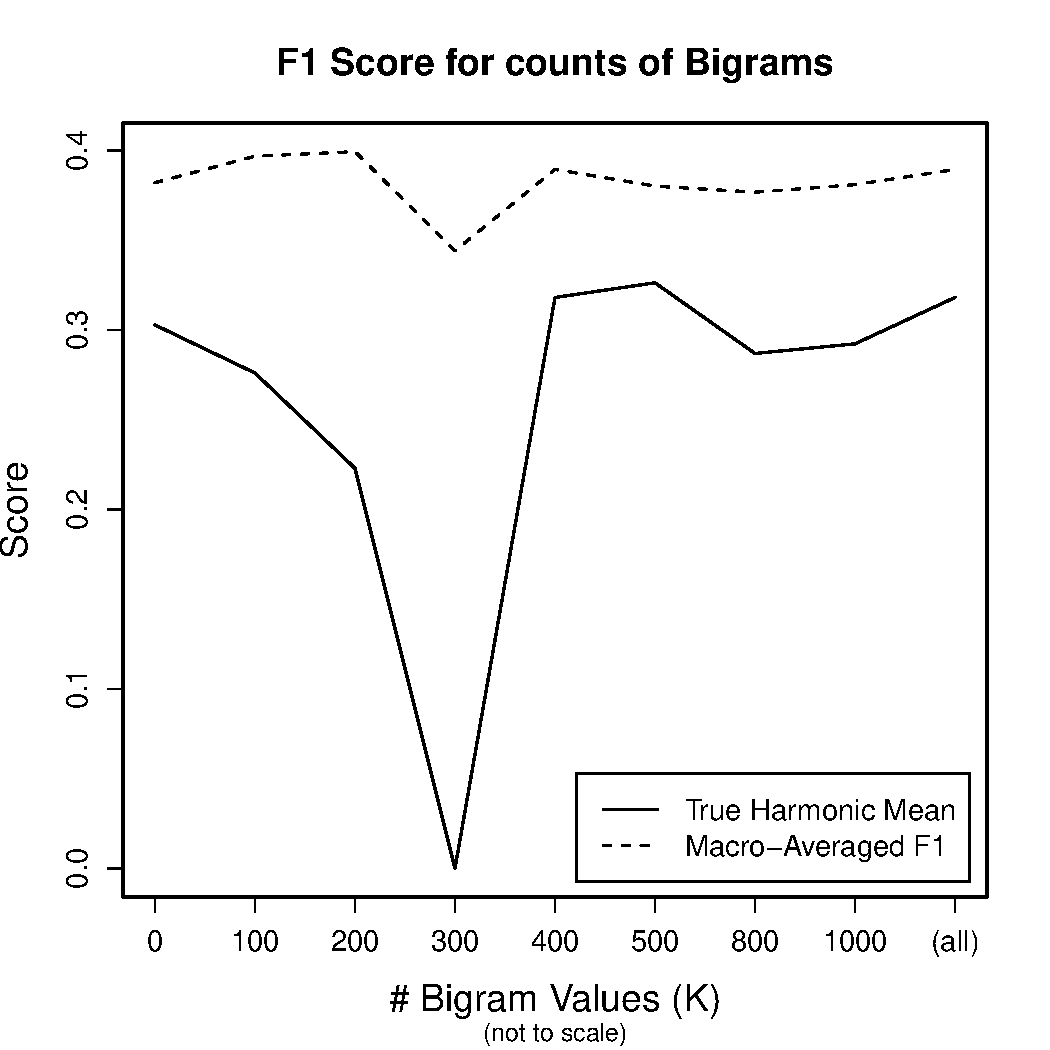
\includegraphics[width=\linewidth]{figs/f1_bigrams}}
\caption{Accuracy metrics for different numbers of baseline *grams on all 13 languages.  To obtain the total number of bigram features, multiple the x-axis value by 3. For instance, at $x=100$, there were 100 untagged bigrams, 100 untagged unigrams, and 100 tagged bigrams.  At {\tt all}, there were a total of 174,125 features.  300 bigram values performed poorly because no users were ever predicted to speak Danish (score of 0 for precision and undefined for recall).}
\label{fig:bigrams}
\end{figure}

Figure~\ref{fig:bigrams} shows the $F1$ scores for a varied number of bigrams, including an experiment with no bigram features at all, and one with features for all 174,125 features (12,936 untagged unigrams, 159,967 untagged bigrams, and 1,222 tagged bigrams).  The accuracy measures in the plot are from training accuracy on all 13 languages, so they can be compared to the numbers of LOOCV found in Table~\ref{tab:loo} with one caveat:  since they were not the result of cross-validation, the accuracy is much higher.  

There are several interesting points about this graph.  Most notably, and as discussed previously, the harmonic $F1$-score calculated in Equation~\ref{eq:harm-f1} is consistently less than that of the macro-averaged $F$ score.  This probably under-estimates the true accuracy statistic, especially because it is {\it extremely} influenced by lower values ($K=300$ bigrams).  

The other interesting point is that, while there is a significant variation between $F$-scores for certain numbers of bigrams (between 300 and 500, for example), there is only a very small difference between using all or no bigrams.  From this, it would appear that, unlike the results obtained by Koppel and Tsur, word bigrams do not play a large part on overall language classification.  Further, while it is possible to make a {\it poor} choice in selecting a number of bigram features (and be heavily penalized in the harmonic $F1$ score), whether one selects 500 or 0 can only account for at most 5\% of the overall accuracy.



\subsubsection{Values of $C$}\label{sec:c}
% Talk about experiments with C

The next experiment we performed was to determine the impact of individual SVM parameters by fluctuating the value of $C$, controlling the tradeoff between training error and margin.  Since it would not make sense to use training accuracy to test this parameter and since it took a significant amount of time to run on the full, 13-language dataset, we used a reduced, 6-language training set with a standard number (500) of bigrams for this experiment.  In addition to determining the optimum value for $C$, this experiment was also designed to identify how classification error was affected by limiting the languages to only those with high support (30 or more users).  

The results for this experiment are in Figure~\ref{fig:C}.  Between individual steps in $C$, the accuracy fluctuates wildly, nearly 5\% difference in some cases.  In spite of this fluctuation, there does appear to be at least a local maximum at $C=0.3$ (the graph drops off quickly with $C=0.2$ and further $0.1$).  After the value of $C=2$, the graph trends upward, but at the extreme cost of time (at $C=1$, a single non-CV training run on all 13 languages took between 5 and 10 minutes; at $C=10$, it did not finish in 3 hours).

These results show that selecting the optimal value of $C$ can be very important.  For example, selecting a value of $C$ at $0.2$ instead of $0.3$ can result in a 6.9\% decrease in the $F1$ score, and the $F1$ score $C=1$ is 5.2\% lower than the optimal.  This is a little disconcerting, as it suggests that specific parameters of the classifier have almost as much impact as the data itself (see Figure~\ref{fig:bigrams}, where, excluding $K=300$ bigrams, the difference between the minimum and maximum is at most 10\%).

\begin{figure}[tb]
\centerline{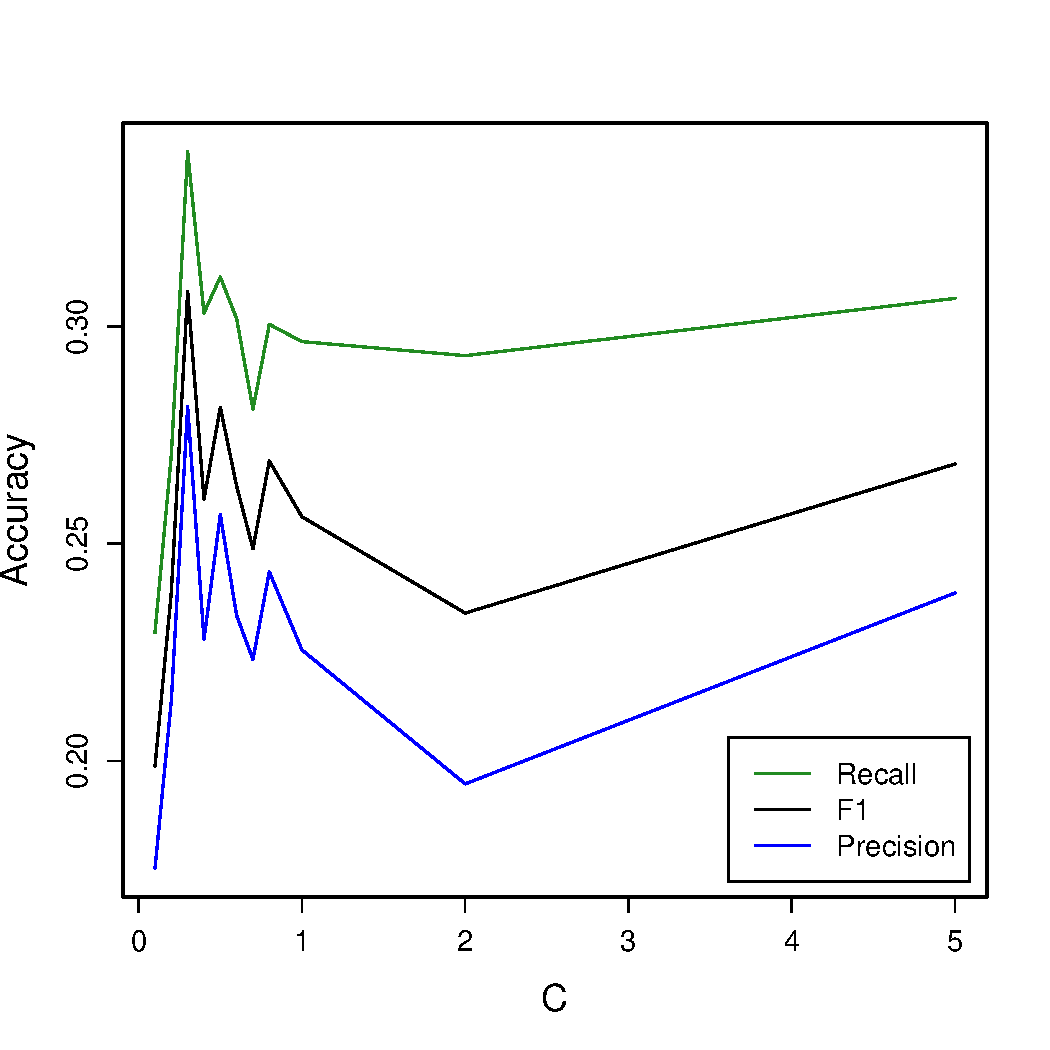
\includegraphics[width=\linewidth]{figs/C_top6}}
\caption{Accuracy metrics for different values of $C$. There appears to be at least a local maximum at $C=0.3$, but with significant variation from value to value.  Scores are the mean of all multi-class values.}
\label{fig:C}
\end{figure}

\subsubsection{Classification Based on Language Family}\label{sec:fam}
After all of our parameter optimizations, we still were not getting quite the accuracy we wanted.  We also noticed some strange trends in the 6-language classifier, and that some languages always performed poorly ({\it Spanish}, for example), even though they generally had a good amount of support.  We thought that this might be due to high similarities between certain families of languages ({\it German} and {\it Dutch} are very close, for example, as are {\it Spanish} and {\it Italian}).  So, for our final experiment, we collapsed these languages in to a single grouping to determine if classification improved on generalized family.  To create a test set, we took the 30 users from the top 6 languages and combined them into three groups:  {\it Germanic}, {\it English}, and {\it Romance}.  We thought it fair to use {\it English} as a separate language ``family'' because this was L1 language attribution, and it theoretically should be trivial to identify someone speaking in their native tongue.  For training and testing with the SVM, we used LOOCV on a feature set with 500 bigrams.

The confusion matrix for this 3-class SVM is found in Table~\ref{tab:top-3}.  Some families tended to be classified very easily---the Romance languages, for example, had an $F1$ of 70\%.  English, on the other hand, did very poorly.  When looking closer at the individual cross-validation results, we noticed a trend:  the first users in each individual language were always classified as {\it Germanic}, and users that came later in the file tended to be classified as {\it Romance}.  We quickly realized that, because the language files were sorted by the number of words each user spoke, the deciding plane for this method of classification was likely based on the number of words each user spoke instead of some intrinsic characteristic of language families.

\begin{table}[t]
\caption{The confusion matrix for language families combined.  While English 
{\it is} a Germanic language with Romance influence, most of the clustering appears to be based on word count rather than intrinsic language properties.}\label{tab:top-3}
\begin{tabular}{r|lll}
& Germanic & English & Romance\\\hline
Germanic & 32 & 0 & 28\\
English & 5 & 0 & 25\\
Romance & 13 & 0 & 77
\end{tabular}
\end{table}  

Further validation of this word-count-biased hypothesis can be found in Figure~\ref{fig:langs}.  Each cell shows a histogram for the number of words used by a given user.  Languages like {\it German} or {\it Dutch} have several users that spoke more than 20,000 words and very few that spoke less than 1,000.  {\it Spanish}, {\it French}, and {\it Italian}, on the other hand, are overwhelmingly influenced by users that spoke 1,000 words or less.

% Talk about why we did not get as good results as we had wanted.  Also include the 3-class results for Germanic vs Romantic languages
\begin{figure}
\centerline{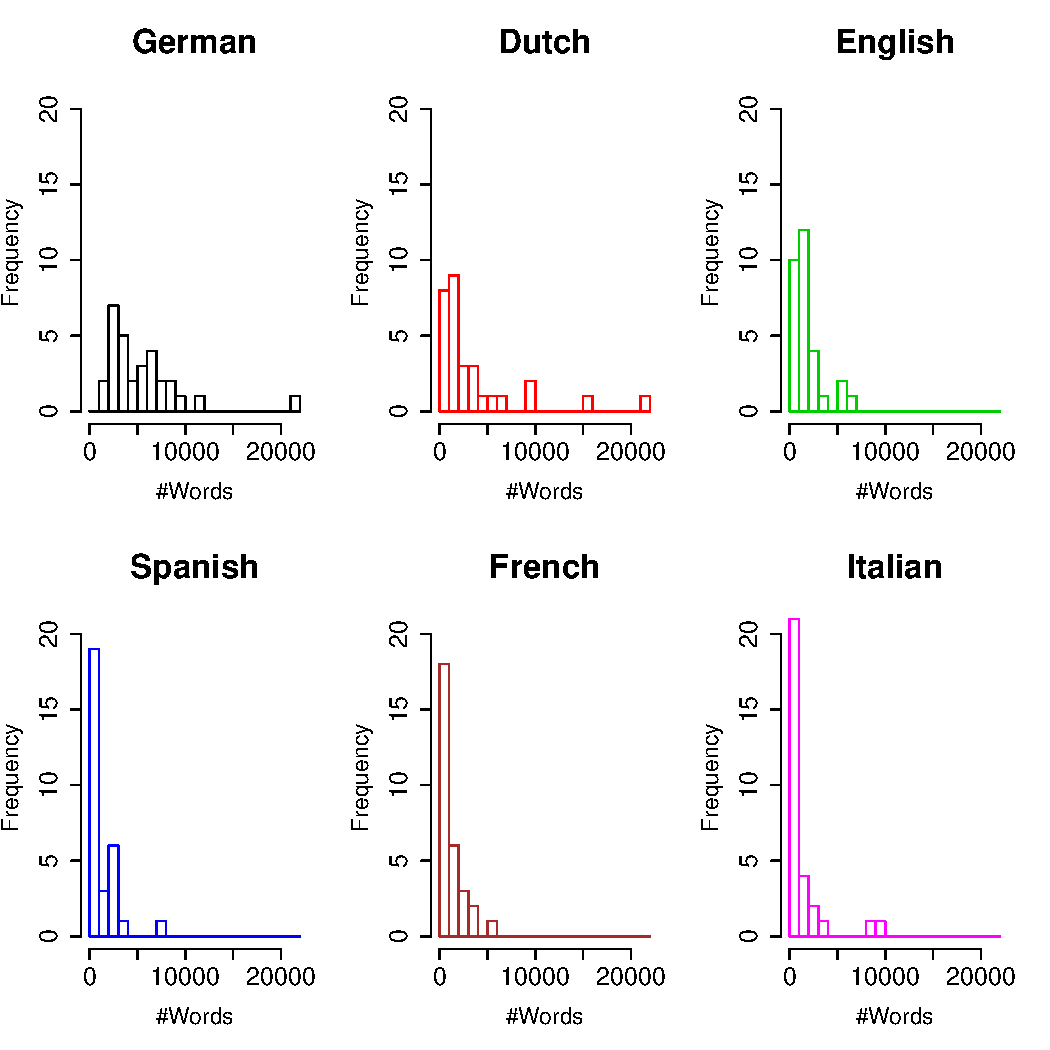
\includegraphics[width=\linewidth]{figs/words_per_lang}}
\caption{The distribution of word counts within languages.  Note that German has a large number of users who spoke a large number of words, whereas French users generally spoke relatively few words.}
\label{fig:langs}
\end{figure}


\subsection{Discussion and Related Work}\label{sec:discussion}
% Is your hypothesis supported? What conclusions do the results support about the strengths and weaknesses of your method compared to other methods? How can the results be explained in terms of the underlying properties of the algorithm and/or the data.

On their own, our results do not seem very positive.  While we are able to outperform the baseline for average guessing at 7.7\% nearly every time (including the overall $F1$ score for the 13-language test and most of the individual $F1$ scores), there seem to be several factors that greatly influence accuracy that are {\it not} attributes of spoken or learned language.  For example, the value of $C$ in the SVM program showed differences greater than 10\%; the difference between using all bigrams and none at all was very small; and, most disconcerting, the three-language classification seemed to label users based upon the number of words they spoke, and not some sort of intrinsic language attribute.  

% This should probably go under Related Work
In spite of these shortcomings, we still feel that our results do compare positively with those already published.  One of the major motivating factors behind doing this research project were comments made in this previous work.  Tsur, et. al. \shortcite{Tsur2007} stated that ``using transcripts of spoken language corpora written in a phonetic script should produce even stronger results'' than that seen both by him and Koppel.  While our corpus did not contain phonetic transcriptions, it is much closer to this ``natural'' language and should produce much better results.  In addition, Brooke et. al. \shortcite{Brooke2012} hammered the results by Koppel and Tsur, saying the data had ``serious issues'' such as the ``confounding factor'' of topic bias in the \emph{ICLE} corpus.  To our knowledge, our corpus does not have this same topic bias.

By just taking the work and comment by Tsur at face value, our peak $F1$ score on the 6-language data of 30.8\% is trounced by their 93.8\% accuracy, and there is no accuracy gained by natural language.  However, we feel that our corpus more closely resembles that studied by Brooke.  When comparing to these latter results, our 6-language F1 score is nearly 6\% better than their 7-language score at 25\%.  In addition, Brooke et. al. showed that by increasing the amount of data, there is a direct increase in the accuracy of each trainer---which means that with a greater number of users, our method should also perform better.

While there are some shortcomings to our data (the corpus was definitely not ``cheap,'' but required numerous man-hours from trained experts), and a few unanswered questions to our methodology remain (described above), there are some features to our corpus and methods that far surpass those done previously.  Most notably, the casual speech of an L2 English speaker will not be altered by editing, grammar checking, and careful consideration of words used.  For these reasons, we feel this is important work that has the potential to determine the basis of {\it ideas} in L2 English speakers.  

%\section{Related Work}
% Answer the following questions for each piece of related work that addresses the same or a similar problem. What is their problem and method? How is your problem and method different? Why is your problem and method better? 

\section{Future Work}
% What are the major shortcomings of your current method? For each shortcoming, propose additions or enhancements that would help overcome it. 
Many of the avenues for future work this research have been discussed previously in this paper.  However, there are a few that should be mentioned here again.

% F1 score---which is correct?  Do we even want to discuss this?  I dunno...

% Address the user word-length issue.  Select several users that have approximately the same number of word utterances.
Obviously, the first (and probably the simplest) avenue for future work is to determine what effect, if any, the number of words a user speaks has on its SVM classification.  To create this dataset, first rank all the users by the total number of words they spoke, then only use those users that are within a reasonable cutoff (remove the 20k+ speakers and those that spoke less than 100 or so).  This might reduce the number of available users for some languages (such as {\it German} and {\it Dutch}), but would maintain a consistency among users that did not exist in this work.  If the results are similar or better, it was probably not due to word count.  If, however, the accuracy degrades significantly, we might conclude that the word usage bias was too strong to overcome.

% Identify if there are differences {\it among} users instead of languages.  Some users talk about soccer.  Does this generally overwhelm the classifier?  Is there a confounding bias between the type of activity this 
Another possible confounding factor that could be unearthed with further work is the degree to which individual {\it users} play in classification.  For example, some users participated in casual conversation on borderline-crude topics, while others were the subject of a press conference for a soccer team.  Is it possible to determine if there are users that naturally cluster together depending on subject or formality of the conversation instead of L1 language?  This is not as easy as removing word bias, but could potentially be done by recording the specific conversations in which each individual was involved and correlating them with predicted languages.

% How does our method perform when tested with other corpora, such as that contained in LANG-8?
The final task that would be a true test of our method's power would be to train the SVMs on the VOICE data, and then test on one of the other corpora---\emph{LANG-8}, for example.  Many of the features would probably need to be removed (such as foreign words and onomatopoetic utterances), but it would be interesting to see how accurate our methods perform on cheap, uncurated data.

\section{Conclusion}
% Briefly summarize the important results and conclusions presented in the paper. What are the most important points illustrated by your work? How will your results improve future research and applications in the area? 
Our work demonstrates some success in applying NLI to novel data. In fact, given the security and intelligence-oriented motivation behind current research, our approach possibly bears more utility than pre-existing work over prompt-driven essay corpora. Moreover, we draw the following conclusions:

\begin{itemize}
\item Our results corroborate the conclusions of Brooke and Hirst \shortcite{Brooke2012}---that the results of previous work on \emph{ICLE} may contain biases unique to that corpus. NLI applied to a ``noisier" corpus yields positive results, though far less significant than those cited by Koppel et. al. \shortcite{Koppel2005a}.
\item Our comparisons to related work verify that NLI techniques similar to those used on text corpora may be applied successfully to transcriptions of speech corpora---with modifications to features as appropriate.
\item Our analysis demonstrates that extemporaneous speech is classifiable through disfluencies and other measures related to spoken word, though it loses the utility of some text-based features, such as orthographic cues garnered by spelling and punctuation variation.
\end{itemize}


\bibliographystyle{acl}
\bibliography{cs388_project}

\end{document}